\documentclass[a4j,fleqn,dvipdfmx,uplatex]{jsarticle}

\usepackage{sice-si}

\usepackage{epic,eepic}
\usepackage[dvipdfmx]{graphics}
\usepackage[dvipdfmx]{graphicx}
\usepackage[dvipdfmx]{color}
% \usepackage{fancyhdr} % ヘッダフッタの罫線と文字出力
% \pagestyle{fancy} % ヘッダフッタの罫線と文字出力(fancyhdrパッケージとセット)
\usepackage{amsmath} % 数式用
\usepackage{amssymb}
\usepackage{tabularx}
\usepackage{enumerate}
\usepackage{txfonts}
\usepackage{url}
% \usepackage{bm}
\usepackage[subrefformat=parens]{subcaption}
\captionsetup{compatibility=false}

% 図表参照に章番号付加 章をまたいでの参照は不可
\newcommand{\figref}[1]{Fig.\ \ref{#1}}
\newcommand{\tableref}[1]{Table.\ \ref{#1}}

% 章番号の後調整
\newcommand{\secref}[1]{\ref{#1}\hspace{0.2zw} 章}
% 節番号の後調整
\newcommand{\subsecref}[1]{\ref{#1}\hspace{0.2zw} 節}

% 画像挿入テンプレ
% \begin{figure}[tb]
%     \centering
%         \includegraphics[width=\linewidth]{img/〇〇〇〇.jpg}
%         \caption{キャプション}
%         \label{ラベリング}
% \end{figure}


\begin{document}
%
% タイトルと著者名
\title{新入社員課題報告書\\[2mm]新社屋屋上室外機における\\散水システム導入および比較検討} % 和文タイトル
\name{○高橋 京佑 (FTE プラント設計部), 2022年新入社員 技術配属者一同} % 著者名
\etitle{} % 英文タイトル
\ename{\small○KEISUKE Takahashi (FoodTechnoEngineering)}	%著者名(英)
%%%%%%%%%%%%%%%%%%%%%%%%%%%%%%%%%%%%%%%%%%%%%%%%%%%%%%%%%%%%%%%%%%%%%%%%%%%%%%%%%%%%%%%%%%%%%%%%%%%
% アブストラクト
\abst
{Recently, "Smart Agriculture" has been promoted in the agricultural sector, but there are issues to be solved in terms of diagnosis technology 
for crop growth and pest invasion. The introduction of multi-spectral sensors will solve these problems. 
"To build a "Spectral Library," we will examine whether it is possible to use UAV to guide flights around the target using "AprilTag."}

% タイトルの出力
\maketitle
%%%%%%%%%%%%%%%%%%%%%%%%%%%%%%%%%%%%%%%%%%%%%%%%%%%%%%%%%%%%%%%%%%%%%%%%%%%%%%%%%%%%%%%%%%%%%%%%%%%
% 本文
\section{序論}\label{sec1}
\subsection{背景}\label{background}
近年, 地球温暖化の影響のため, 日本全国の気温は上昇傾向にあり, 
2021年の大阪府の年間平均気温は1883年に比べ2.5℃上昇している\cite{temp_osaka}. 
さらに, 2021年の真夏日と猛暑日の合計日数は, 2014年の65日に比べ13日増加, 
猛暑日に関しては8日増加しており\cite{temp_osaka2}, 1880年からの真夏日および
猛暑日の長期的推移を見ると増加傾向である\cite{temp_osaka3}. 


\begin{figure}[tb]
    \centering
    \begin{minipage}[b]{\linewidth}
      \centering
      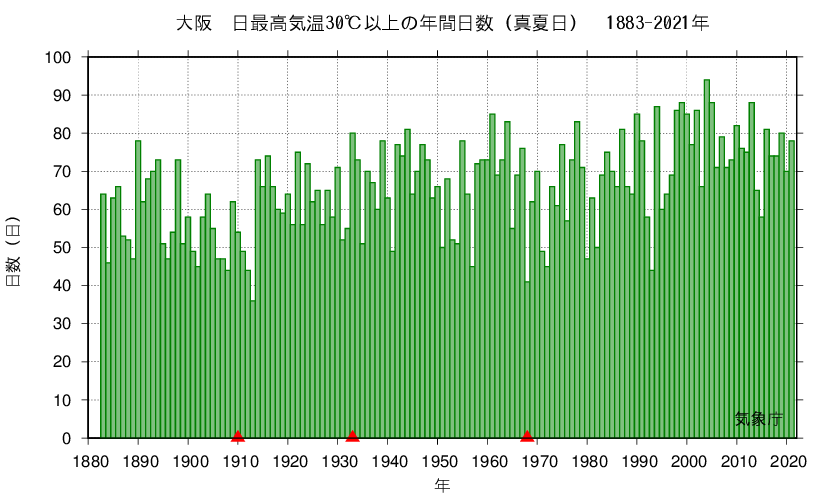
\includegraphics[width=\linewidth]{img/27_OSAKA_tmaxGE30_2021.png}
      \subcaption{真夏日}
      \label{subfig1:temp_osaka}
    \end{minipage}\\
    \begin{minipage}[b]{\linewidth}
      \centering
      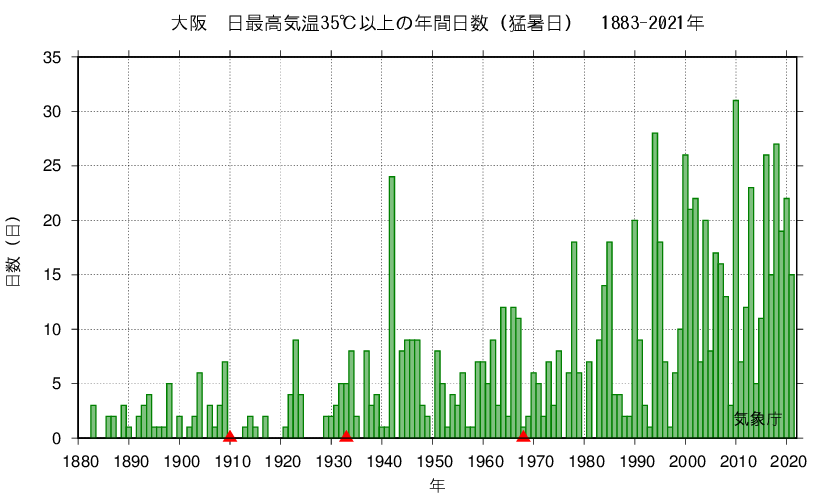
\includegraphics[width=\linewidth]{img/27_OSAKA_tmaxGE35_2021.png}
      \subcaption{猛暑日}
      \label{subfig1:temp_osaka2}
    \end{minipage}
    \caption{大阪府気温推移}
    \label{fig1:temp_osaka}
\end{figure}


\subsection{目的}\label{purpose}
% \subsecref{background} で前述した「スペクトルライブラリ」構築のため, \figref{fig:spectrum}のようにUAVを測定対象を全方位から撮影できるよう飛行させる必要がある. 
% その際に測定対象周辺に基準マーカーを配置し, カメラでスペクトル計測時もしくは経路移動中常に計測対象とマーカーを同時に捉えておくことで正確に計測対象を撮影できると考えた. 

% 現在, 指定された経路に従ってUAVが移動するためには, Way Point (以下,WP)を設定し, GPSの情報を利用してWP上を移動する方法が一般的である\cite{WP}. 
% しかしながら, GPSベースのWPナビゲーションによる飛行はGPS受信数が多い環境である上に,計測対象の正確な緯度・経度情報をUAVに対して指示する必要があり, そのオペレーションは煩雑である.
% 従って,本研究では誰でも使いやすいシステムによってスペクトルライブラリを構築するために,基準マーカー(Fiducial Marker, マーカー)を測定対象周辺に設置することによる
% 飛行精度を向上させる手法を考察することを目的とする. 

% \begin{figure}[tb]
%     \centering
%         \includegraphics[width=\linewidth]{img/asset5.jpg}
%         \caption{太陽 - 計測対象 - センサ(UAV)の位置関係}
%         \label{fig:spectrum}
% \end{figure}

\section{調査内容}\label{sec2}

\subsection{DIY}\label{subsec:apriltag}

\subsection{配置条件}\label{subsec:tag_pos}



\section{実験}\label{sec3}

\subsubsection{M600のハードウェア構成}\label{subsubsec:m600}


\subsubsection{M300のハードウェア構成} 


\subsubsection{ソフトウェア構成}


\subsection{実験1: GPSのみを用いた飛行実験}\label{subsec:ex1}

\subsection{実験2: AprilTagによる位置補正}\label{subsec:ex2}

\subsection{実験3: AprilTagの位置精度の検証}\label{subsec:ex3}

\begin{table}[h]
\caption{AprilTagの位置精度}
\label{table:tag_pos}
\centering
\begin{tabular}{lrrrrr}
    & 実験3-1 & 実験3-2 \\
    \hline \hline
    Tag0 & 76.88\% & 97.22\% \\
    Tag1 & 73.03\% & 95.05\% \\
    Tag2 & 82.87\% & 91.30\% \\
    Tag3 & 75.00\% & 87.33\% \\
    \hline
\end{tabular}
\end{table}


\section{考察}


\section{結論}

\section{緒言}
本稿では SICE SI 部門講演会 SI2021 の予稿原稿を作成するための説明を行います.
SI2021では予稿原稿としてPDFファイル形式のファイルを電子投稿していただくことを原則とさせていただいております.
ただし,電子化やネットワーク接続が困難な場合には個別に対応させていただきますので,プログラム委員会までご相談ください(Webサイトからお問い合わせできます).
%
\section{原稿作成方法}
\subsection{原稿枚数,ファイル形式とファイル容量}
原稿は1講演につき1ページから最大6ページとなります(キーノート講演も同様です).
提出していただく原稿のファイル形式は原則としてPDF形式といたします.
PDF形式とすることが不可能な場合には,プログラム委員会にご連絡ください.
また,原稿完成時のファイルサイズはPDF形式で2MB程度を上限の目安とさせていただきます.
原稿送付時にはそれ以上でも受付可能な場合がありますが,その場合には全体の原稿の総容量により再提出をお願いする場合がありますので,ご了承ください.
%
\subsection{用紙サイズ,書式など}
\subsubsection{原稿の体裁}
用紙サイズはA4版(縦297mm$\times$横210mm)とし,余白部分は左右15mm,上20mm,下27mmを確保してください.(プログラム委員会でヘッダ・フッダ部分に情報を追加する予定ですので,ご注意ください.)
よって,原稿作成領域は250mm$\times$180mmの枠内となります.
%
\subsubsection{基本書式}
原稿の記載内容は,下記の順序とします.
\begin{enumerate}
\setlength{\parskip}{0cm} % 段落間詰める
\setlength{\itemsep}{0cm} % 項目間詰める
\item[1)] 和文題目(英文原稿の場合には不要,16ptゴシックフォント推奨,センタリング)
\item[2)] 和文著者名・所属(英文原稿の場合には不要,12pt明朝フォント推奨,センタリング,登壇者に○を付加)
\item[3)] 英文題目(16pt Times-Roman Bold推奨,センタリング)
\item[4)] 英文著者名・所属(12pt Times-Roman推奨,センタリング,登壇者に○を付加)
\item[5)] 英文アブストラクト(9pt Times-Roman推奨,3 〜 5行程度,文章両側を10mm程度インデント)
\item[6)] 本文(本文文章は10pt明朝フォント推奨,小見出しは12 〜 10pt程度のゴシックフォント推奨)
\item[7)] 参考文献(10pt明朝フォント推奨)
\end{enumerate}
\subsubsection{図と表について}
予稿はPDFファイルとなりますので,図や表はカラーで作成していただいても構いません.
ただしファイルサイズの制限にご注意ください.
図のキャプションは図の下にFig.1,Fig.2という具合に,表のキャプションは表の上にTable 1,Table 2という具合にお付けください.(英語表記,フォントは10pt Times-Roman推奨)
%
\section{結言}
本稿はあくまでも予稿原稿を作成するためのガイドラインを示したものです.改行幅やフォントの設定などについては,原稿の内容や量に合わせて適宜判断していただき,原稿を作成してください.
また,本稿はSICE-SI2021の予稿原稿の書き方\cite{SI2021}を参考に,\TeX 用書式を用意したものです.適宜sice-si.styを変更して使用してください.


%参考文献
\begin{thebibliography}{99}
\bibitem{temp_osaka}
国土交通省, 気象庁, 大阪府 日最高気温の月平均値, 
\url{https://www.data.jma.go.jp/obd/stats/etrn/view/monthly_s3.php?prec_no=62&block_no=47772&year=&month=&day=&view=a2}\vspace{2mm}

\bibitem{temp_osaka2}
George's Web Sites, 大阪府-大阪市の気温に関する統計情報, 
\url{http://www.tvg.ne.jp/george/weather/gw_stat_temp.html?city=oosaka}\vspace{2mm}

\bibitem{temp_osaka3}
A-PLAT 気候変動適応プラットフォーム, 気候変動の観測・予測データ, 大阪府観測データ, 
\url{https://adaptation-platform.nies.go.jp/map/Osaka/index_past.html}\vspace{2mm}
\end{thebibliography}
%
%
%
\end{document}